\section{Akteure und Anwendungsfälle}

CardHub hat vier Akteure. Der \textbf{Gast} ist nicht angemeldet. Er legt ein Konto an oder meldet sich an. Der \textbf{Sammler} ist angemeldet und der primäre Akteur. Ein \textbf{Freund} ist ein Sammler mit bestätigter Freundschaft. Er tritt erst im Ausbau auf. Der \textbf{API-Aufrufer} ist ein technischer Akteur. Er startet regelmäßig den Import von Kartendaten und Preisen aus der TCGdex-API. Kamera und Erkennungsmodell gehören zur App und sind keine Akteure.

\begin{figure}[H]
\centering
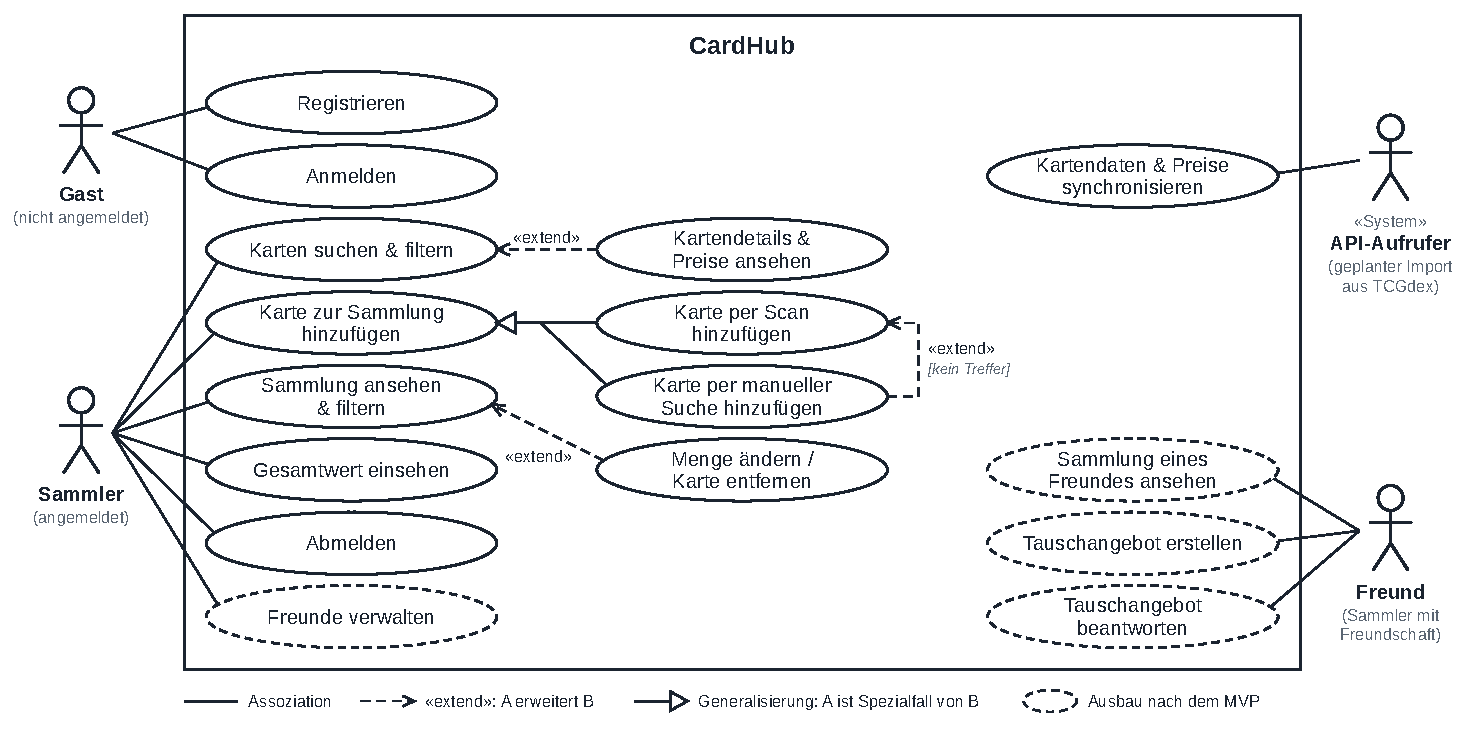
\includegraphics[width=\linewidth,height=8.2cm,keepaspectratio]{diagramme/usecases.pdf}
\caption{Use-Case-Diagramm für MVP und Ausbau. Eigene Darstellung.}
\label{fig:usecases}
\end{figure}
\subsection{Anwendungsfälle im Überblick}
Abbildung~\ref{fig:usecases} zeigt alle Anwendungsfälle. Nach der Anmeldung handelt der Gast als Sammler. Der Sammler sucht Karten im Katalog und filtert nach Set oder Typ. Kartendetails und Preise erweitern die Suche. Karten fügt er per Scan oder per manueller Suche hinzu. Beide Wege sind Spezialfälle von \emph{Karte zur Sammlung hinzufügen}. Die manuelle Suche erweitert den Scan, wenn kein Vorschlag passt. In der Sammlung ändert er Mengen oder entfernt Einträge. Der Gesamtwert summiert die Richtwerte.

Im Ausbau verwaltet der Sammler seine Freunde. Ein Freund sieht freigegebene Sammlungen und erstellt ein Tauschangebot. Der Empfänger nimmt es an, lehnt es ab oder stellt ein Gegenangebot.

\subsection{Hauptanwendungsfall: Karte per Scan hinzufügen}
\textbf{Vorbedingung:} Der Sammler ist angemeldet und hat die Kamera freigegeben. \textbf{Ablauf:} (1)~Der Sammler startet den Scanner und nimmt die Karte auf. (2)~Das lokale Modell ermittelt bis zu fünf Kandidaten. (3)~Der Sammler wählt den Treffer und legt die Anzahl fest. (4)~Die App sendet Karten-ID und Anzahl an das Backend. (5)~Nach der Bestätigung des Servers zeigt die App den Eintrag. \textbf{Alternativen:} Passt kein Kandidat, sucht der Sammler die Karte manuell. Bei einem Netzfehler bleibt die Auswahl erhalten. \textbf{Ergebnis:} Die Sammlung enthält die Karte mit positiver Anzahl.

\subsection{Folgerungen für Software-Design und Technologie-Stack}
Der Scan läuft auf dem Gerät. Die App braucht Kamera und lokales Modell auf Android und iOS. Die Sammlung ist geschützt. Ein zentrales Gateway prüft bei jeder Anfrage die Anmeldung. Katalog und Preise liefert ein Fremdsystem. Ein eigener Dienst importiert sie. Mengen und späterer Tausch verlangen konsistente Bestände. Dafür eignet sich eine relationale Datenbank mit Transaktionen.
